\documentclass[12pt,a4paper]{report} %How the pages are set up
\usepackage[danish]{babel} %set which langue the name of things are
\usepackage{fancyhdr} %package to change the headder and fotter
\usepackage{lastpage} %package to be able to reference the pagenumber of the last page
\usepackage{tocloft} %package to change the formating of the table of contents
\usepackage{hyperref} %package to put links in the pdf (and make the table of contents lines to links to the respective lines)
\usepackage{color} %package to have a static reference to colors
\usepackage{titlesec} %package to change the formatting of the titles
\usepackage{datetime} %package to reference the current date and time
\usepackage[pdftex]{graphicx} %package to set default layout when compiling
\usepackage[utf8]{inputenc} %package to set the typeset
\usepackage{gensymb} %package to add some mathematical symbols
\usepackage{cite} %package to be able to quote stuff
\usepackage{enumitem} %package to change formatting of lists
\usepackage{rotating} %package to be able to rotate figures
\usepackage{caption}%package to add captions to pictures
\usepackage{longtable}%package to make tables that span multiple pages
\usepackage{listings}
\usepackage{hyperref}
\usepackage{atbegshi}
\usepackage{pdfpages}
%\renewcommand\bibname{Kildehenvisning}


\AtBeginDocument{\AtBeginShipoutNext{\AtBeginShipoutDiscard{}}}
\addto\captionsdanish{
  \renewcommand{\bibname}
    {Kildehenvisning}
}

\addto\captionsdanish{
  \renewcommand{\contentsname}
    {Indholdsfortegnelse}}

\addtocontents{toc}{\protect\thispagestyle{empty}}
\setlength{\parindent}{2em}
\linespread{1.2}
\setlist[itemize]{itemsep=0mm}
\definecolor{gray75}{gray}{0.75}
\newcommand{\hsp}{\hspace{20pt}}
\titleformat{\chapter}[hang]{\Huge\bfseries}{\thechapter\hsp\textcolor{gray75}{$|$}\hsp}{0pt}{\Huge\bfseries}
\titlespacing*{\chapter}{0pt}{-50pt}{40pt}
\setlength{\parskip}{1em}
%\renewcommand{\headsep}{-3em}

\title{
    \vspace{2em}\newline 
    Gruppe 25
}
\author{
\resizebox{\columnwidth}{!}{
\begin{tabular}{ccc}
Rasmus . .                             & Philip B. Ø.,                  & Michael J.,                           \\
s185129                                  & s185146                         & s185123                               \\
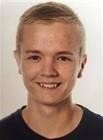
\includegraphics{Billeder/personer/AndersBjoerndalPedersen.jpg}&
\includegraphics[]{Billeder/personer/PhilipBocayesOernskov.jpg}&
\includegraphics[]{Billeder/personer/MichaelJeppesen.jpg}\\
\newline
                             &Nicklas C. F.,                                         \\
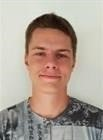
\includegraphics[]{Billeder/personer/NicklasChristofferFritzen.jpg}
\end{tabular}}
}
\date{\vspace{-1em}\hspace{4em}\today\newline
GitHub url: \url{https://github.com/Fipzz/Compilerteknik---Assingment-1}

\pagestyle{fancyplain}
\fancyhf{}
\fancyhead{}
\fancyfoot{}
\fancyhead[C]{CDIO FINAL}
\fancyhead[L]{Grp 25}
\fancyhead[R]{\today}
\fancyfoot[C]{Side \thepage\ af \pageref{LastPage}}
\fancyfoot[R]{Gruppe 25}

\fancypagestyle{firstpage}{%
  \lhead{
\includegraphics[scale=0.1]{Billeder/Bilag/DTU_Logo_Corporate_Red_CMYK.png}}
  \rhead{}
}

\documentclass[12pt]{book}
\usepackage{lipsum}

\usepackage{suffix}

\newcommand\chapterauthor[1]{\authortoc{#1}\printchapterauthor{#1}}
\WithSuffix\newcommand\chapterauthor*[1]{\printchapterauthor{#1}}

\makeatletter
\newcommand{\printchapterauthor}[1]{%
  {\parindent0pt\vspace*{-25pt}%
  \linespread{1.1}\large\scshape#1%
  \par\nobreak\vspace*{35pt}}
  \@afterheading%
}
\newcommand{\authortoc}[1]{%
  \addtocontents{toc}{\vskip-10pt}%
  \addtocontents{toc}{%
    \protect\contentsline{chapter}%
    {\hskip1.3em\mdseries\scshape\protect\scriptsize#1}{}{}}
  \addtocontents{toc}{\vskip5pt}%
}
\makeatother



\begin{document}
    \begin{titlepage}
    \centering
    \pagestyle{firstpage}
    \maketitle
    \tableofcontents
    \thispagestyle{empty}
    \end{titlepage}
    
    \chapter{Timeregnskab}
    \chapterauthor{Anders R.R (s185146)}
    
    \begin{center}
        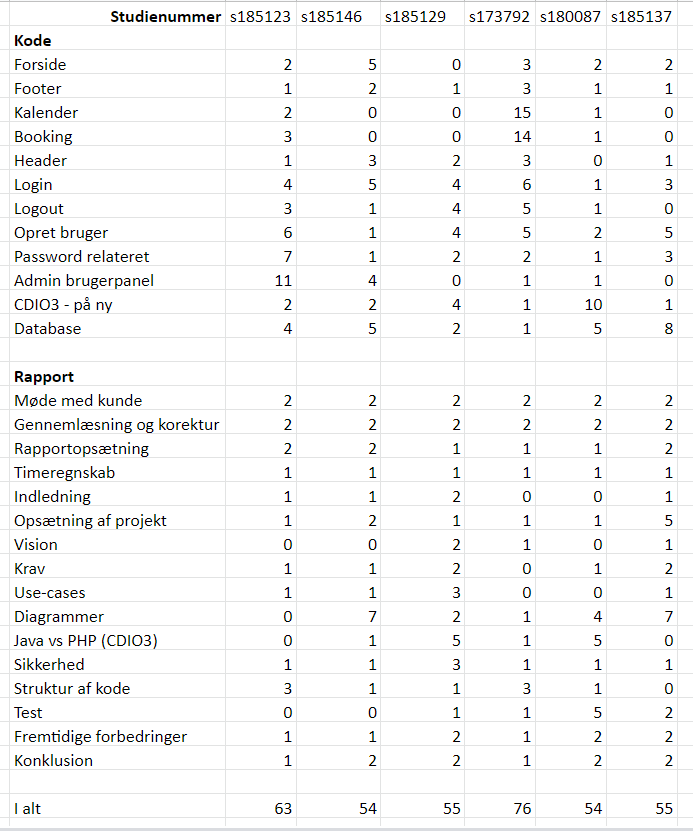
\includegraphics[width=\textwidth]{Billeder/setup/Timeregnskab.PNG}
    \end{center}
    
    \chapter{Indledning}
    \chapterauthor{Anders B.P (s185129)}
    Vi har i dette projekt valgt at lave et specialprojekt i samarbejde med FDF K23 Valby. De har ønsket at få udarbejdet en hjemmeside, hvor de kan administrere udlejning af trailere og mødelokaler. 
    Vi har i denne forbindelse sat os for som opgave, at udvikle en hjemmeside, som opfylder de kravspecifikationer, vi i samarbejde med FDF K23 Valby har udarbejdet.
    Vi har valgt at gribe opgaven an ved først, at holde et møde med FDF K23, for at afgrænse og definere helt præcist hvilke krav og use cases deres hjemmeside skal opfylde og understøtte. 
    \newline
    \newline Herefter har vi undersøgt hvilke teknologier der vil give bedst mening at anvende til udarbejdelsen af det færdige produkt. Vi har her fundet frem til at det ville give bedst mening at anvende programmeringssproget PHP, da det ville spare os for en del linjer kode, modsat at lave det i Java. Derudover er PHP også et nem og intuitivt programmeringssprog når man taler om web-udvikling. Det minder nemlig meget om java, men er langt nemmere at eksekvere med på en webserver. Herudover har vi valgt at koble en MySQL database på vores applikation, da vi i tidligere kurser har stiftet kendskab med MySQL. 
    \newline
    \newline Efter at have fastlagt de teknologier vi ville arbejde med, har vi forsat vores arbejdsprocess med at lave en detaljeret analyse af kravspecifikationer og use cases. 
    \newline Med et solidt fundament fra vores analysefase, er vi gået videre til designfasen. Her har vi fastlagt hvordan strukturen af vores applikation ville se ud. Vi startede med at researche og drage inspiration fra andre lignende projekter, hvor vi bla. fandt frem til de libraries vi ville anvende i forbindelse med de funktioner vores applikation skulle opfylde. Herudover har vi også draget inspiration til udsmykningen af vores hjemmeside, hvor vi besluttede os for at anvende Bootstrap til den visuelle opbygning af vores hjemmeside. 
    \newline 
    \newline Efter designfasen kunne vi påbegynde selve implementeringen af vores applikation. Vi har særligt haft fokus på at opbygge strukturen af vores program fornuftigt for at opfylde principperen og low-coupling og high-cohesion. Dette er gjort for at opdele de forskellige ansvarsområder i vores kode, så vi nemt kan genanvende kode, samt generalt opbygger kode med en fornuftig struktur. 
    \newline Et krav vi fik specificeret af kunden var at sikkerheden i applikationen skulle være i top, som er særdeles vigtigt for et moderne website. Vi har derfor implementeret de rette midler for at tage hånd om dette problem såsom bestemte hashing teknikker og taget forbehold for SQL-injections
    
    \newline \noindent Til sidst har vi også købt et domain hos webdomain.dk, da vores endelige produkt skal tages i brug af en reel kunde. 
    \newline
    \newline Vores domain kan tilgås på http://fdfcdio.dk
    
    \newline
    \noindent Eftersom vi har valgt at skrive vores projekt i PHP i stedet for Java, har vi her ved lagt vores CDIO 3 projekt, ved siden af vores færdige projekt-mappe, skrevet i både Java og PHP. Dette er gjort for at vise forskellen på, hvormange linjer kode der kræves i de 2 forskellige sprog, og dette er også en grundende til at vi valgte at skrive vores endelige projekt i PHP fremfor Java. 
    
    \chapter{Vejledning til downloading og opsætning af projekt}
    \chapterauthor{Philip B. Ø. (s185137)}
    
    Da vi anvender PHP, hvilket er et server side programmingssprog, skal man gøre brug af server. Derfor skal man kunne hoste en lokal webserver. Vi anbefalder at anvende XAMPP. \newline XAMPP sørger både for egen hosting på localhost(hjemmeside), og en mysql-database, hvilket er det vi bruger, og det kan hentes vha. Dette link \url{https://www.apachefriends.org/download.html} 
    
    \noindent Når man har hentet og installeret XAMPP, skal projektet ligges i mappen \newline C:\textbackslash xampp\textbackslash htdocs. Efter at have placeret vores projekt i htdocs kan man åbne og kører vores projekt lokalt. Herefter anbefales det at opsætte en lokal MySQL database, kan også køres igennem XAMPP, hvorefter man opretter tables og poulater dem, for at få noget reelt testdata. Dette vises i følgende afsnit. \newpage
    \noindent På nedstående billede vises hvordan XAMPP ser ud, her er det vigtgt at starte den lokale SQL server og Apache server, før vores projekt kan køres lokalt. 
    
    \hspace*{-1.5cm}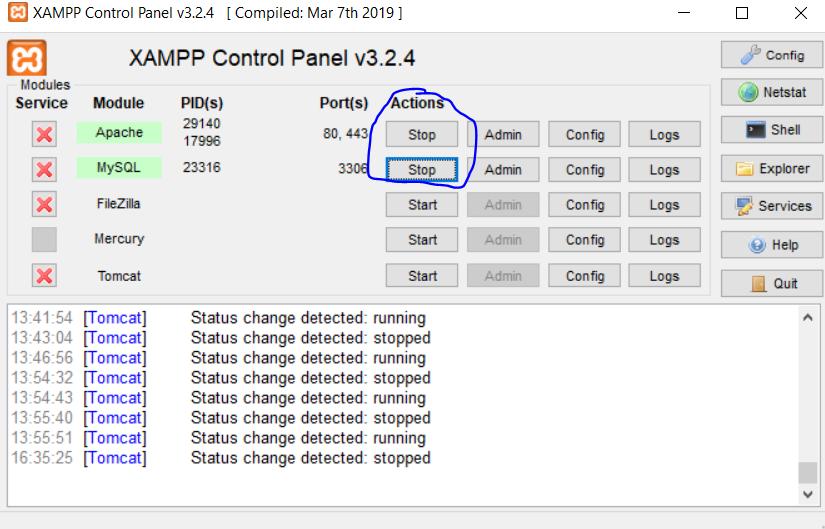
\includegraphics[scale=0.85]{Billeder/installTurtorialPictures/Servers.PNG}
    
    \noindent Efter at have lagt vores projekt i C:\textbackslash xampp\textbackslash htdocs, kan man nu indtaste
    \newline
    \newline
    http://localhost/FDF/FDF20\%Booking/web/forside.php
    \newline
    \newline
    i webbrowseren, og man vil derefter blive mødt af vores forside. 
    
    \noindent Vores afleverede projekt er opsat til at oprette forbindelse til databasen, som kører lokalt på ens egen computer. Dvs. at hostname er localhost, user er root, password er tomt og database navnet er sat til test. På vores egentlige domæne er disse informationer ændret til de korrekte oplysninger i forhold til databasen der er hostet på vores webserver. 
    
    \noindent Vi skal nu til at opsætte en lokal database som vores projekt vil connecte til. Ved at klikke på "admin" ud for MySQL åbner du phpmyadmin som kan bruges til at konfigurere din lokale database.
    
    \noindent Her skal du navigere til databasen "test". klik på den som vist på billdet under.
    
    \hspace*{-1.5cm}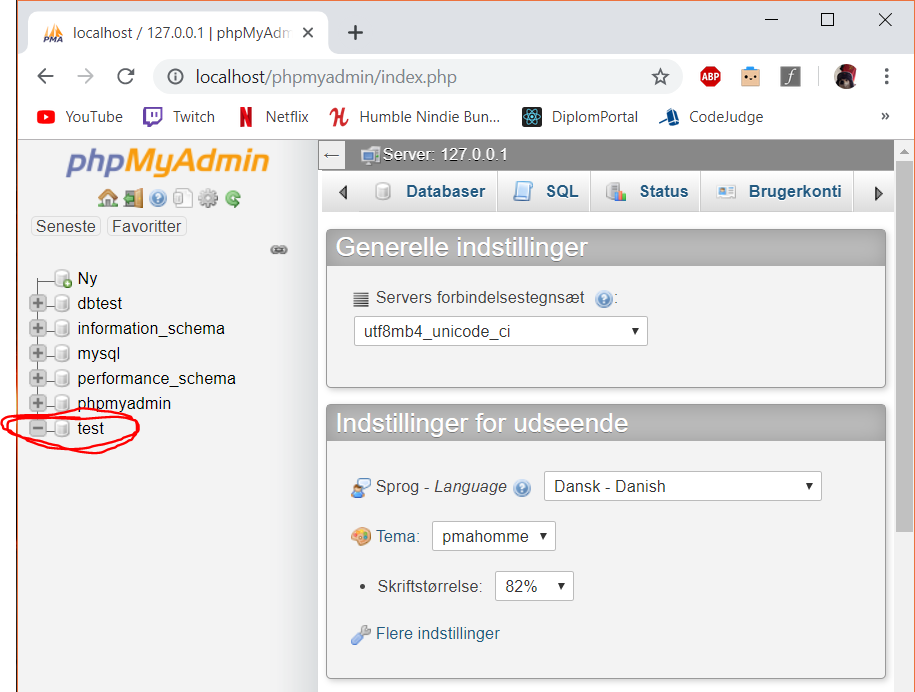
\includegraphics[scale=0.85]{Billeder/installTurtorialPictures/findtestdbrigtig.PNG}
    
    
    \noindent Klik nu på databasen og derefter på "SQL" øverst. Herind skal du køre vores mysql scripts som kan findes under vores resource(res) mappe i vores projekt. Først skal du køre "createTables", og derefter "populateTables".\\\\ Dette kan gøres med copy paste fra filerne.
    
    \hspace*{-1cm}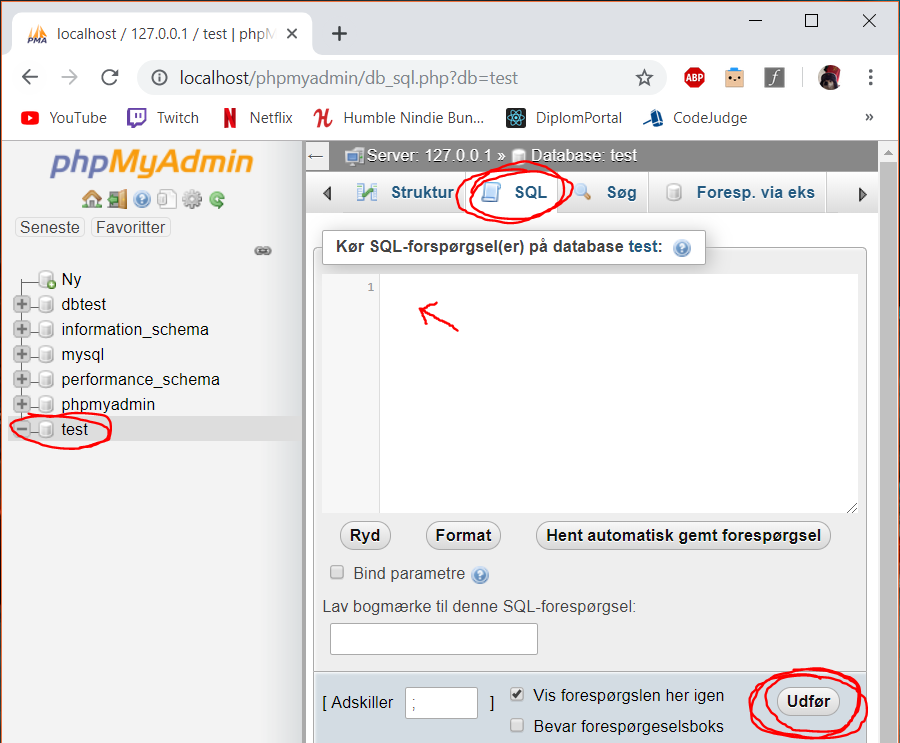
\includegraphics[scale=0.8]{Billeder/installTurtorialPictures/Mysql.PNG}
    
    \noindent For at kunne tilgå vores hjemmeside skal du kunne logge ind. Med den givende populateTables er der sørget for en admin bruger. user='admin', pass='admin' som kan logges ind med og til gå admin rettighederne. Ønsker man at se vores hjemmeside fra en brugers perspektiv bruger man: user='theduck', pass='ripraprup'.
    
    \noindent Når vi skal fremlægge vores 3 ugers projekt, vil det både være lokalt og på internetet. For at kører den lokale version skal man bruge ovenstående vejledning. Hvor den online del er tilgængelig på \url{fdfcdio.dk}
    
    \chapter{Analyse}
    \chapterauthor{Anders B.P (s185129)}
    
    \section{FDF klubbens vision}
    
    FDF K23 Valby er en spejderklub som har omkring 100 medlemmer på nuværende tidspunkt. Klubben har derudover også to trailere og to mødelokaler, som stilles til rådighed for klubbens medlemmer. Klubben ønsker i den sammenhæng at få udviklet en webbaseret løsning, hvor medlemmerne kan reservere trailere og mødelokaler. 
    Klubben ønsker en løsning hvor man kan oprette en bruger og slette en bruger. En bruger skal have mulighed for at booke trailere eller mødelokaler, redigere en booking, slette en booking, vise alle bookinger, samt have en form for administrator panel. For at oprette en bruger ønsker spejderklubben at have en adminkonto, som skal validere nye brugere før de bliver oprettet i databasen.
    Herudover ønsker kunden en simpel og intuitiv løsning, da målgruppen for løsningen primært er ældre personer, eller personer som ikke har meget erfaring med computere. 

    \newpage
    \section{Krav}
    
    Vi har i samarbejde med FDF klubben, fået specificeret nogle krav til denne hjemmeside, ud fra hvilke ønsker de havde til funktionalitet og deres behov.
    
    \subsection*{Funktionelle krav}
    Hjemmesiden skal understøtte følgende krav:
    \begin{itemize}
        \item Oprettelse af brugere
        \item Redigering af brugere
        \item Læsning af brugere
        \item Sletning af brugere
        \item Opretning af lejemål
        \item Redigering af lejemål
        \item Læsning af lejemål
        \item Sletning af lejemål
        \item Oprettelse af booking
        \item Redigere af booking
        \item Læsning af booking
        \item Sletning af booking
        \item Visuel kalender hvor brugere kan se hvornår en trailer/mødelokale er ledigt eller optaget.
    \end{itemize}
    \newpage
    \subsection*{Ikke-funktionelle krav}
    Målgruppen for vores hjemmeside er forholdsvis ældre mennesker, eller personer som ikke besidder den store tekniske snilde, og derved skal vores hjemmeside være nem at finde rundt i, og simpel at betjene.
         For at opnå disse mål, skal vores hjemmeside opfylde følgende krav for at sikre os hjemmesiden bliver nem at anvende.
    \begin{itemize}
        \item Man kan tilgå alle funktioner på hjemmesiden indefor 2 klik
        \item Hjemmesiden skal være responsive, så den kan åbnes og læses på forskellige devices med forskellige aspect-ratioer
        \item Hjemmesiden skal loade på under ét sekund.
    \end{itemize}
        
    \newpage
    \section{Use-cases}
    Vi har følgende use-cases for dette projekt for hjemmesiden. Disse use-cases er udarbejdet ud fra vores kravanalyse, som vi har lavet i samarbejde med FDF K23.
    
    \begin{itemize}
        \item \textbf{Opret bruger\newline}
        Et medlem af klubben skal kunne oprette sig som bruger på hjemmesiden, ved at udfylde en opret bruger-formular med relevante oplysninger. Herefter skal en administrator godkende brugeren, før brugeren bliver oprettet i databasen. 
        \begin{itemize}
            \item En bruger skal angive fornavn, efternavn, telefonnummer, emailaddresse og kodeord i opret bruger-formularen
            \item Hvis en angivet email allerede findes i databasen får brugeren en besked om at emailen allerede er i brug, og brugeren oprettes ikke. 
            \item Hvis et angivet telefonnummer allerede findes i databasen får brugeren en besked om at nummeret allerede er i brug, og brugeren oprettes ikke. 
            \item Når en bruger har udfyldt de nødvendige oplysninger, får brugeren en besked om at hans registering afventer godkendelse, af en administrator. 
        \end{itemize}
        \item \textbf{Godkend ny bruger\newline}
        En administrator skal have mulighed for at godkende nye brugere, før de har adgang til at booke lejemål. Hvis man er logget ind med en administrator-konto skal man have mulighed for at få vist en liste over alle brugere i systemet. Her skal administratoren manuelt godkende nye brugere, før de kan booke lejemål på hjemmesiden. 
        
        \item \textbf{Rediger bruger (bruger)\newline}
        En bruger skal have mulighed for at ændre sine egne oplysninger.
        \begin{itemize}
            \item En bruger skal have mulighed for at ændre sit fornavn, efternavn, telefonnummer, emailaddresse og password.
            \item Hvis brugeren ændre sin email eller telefonnummer til noget der allerede eksisterer i databasen, får brugeren en meddelse om at det ikke kan lade sig gøre. 
            \item Hvis de indtastede informationer er gyldige ændres oplysningerne i databasen, og brugeren får en meddelse om at brugerens oplysninger nu er ændret og gemt. 
        \end{itemize}
        \item \textbf{Rediger bruger (administrator)\newline}
        En administrator skal have mulighed for at ændre i andre brugeres oplysninger.
        \item \textbf{Slet bruger (bruger) \newline} 
        En bruger skal have mulighed for at slette sig selv fra databasen.
        \item \textbf{Slet bruger (administrator) \newline}
        En administrator skal have mulighed for at slette brugere fra databasen.
        \item \textbf{Opret booking\newline}
        En bruger eller en administrator skal kunne oprette en ny booking af trailere og/eller mødelokaler. 
        \begin{itemize}
            \item Hvis en bruger eller administrator forsøger at oprette en booking på en allerede optaget dato, skal brugeren have en besked om at booking mislykkedes, og at den valgte dato optaget.
            \item Hvis en bruger eller administrator forsøger at oprette en booking på en gyldig dato, skal traileren/mødelokalet blive reseveret i det valgte tidsrum, og dette skal derefter også fremgå visuelt på vores kalender. 
        \end{itemize}
        \item \textbf{Rediger booking (bruger)\newline}
        En bruger skal kunne rediger tidspunktet for en booking som han selv har oprettet.
        \begin{itemize}
            \item Hvis en bruger forsøger at ændre tidspunkt til en dato der allerede er booket, får brugeren en fejlmeddelse, og bliver bedt om at vælge en ny dato. 
            \item Hvis en bruger ændre til en gyldig dato ændres udlejningstidspunktet i databasen, og det bliver også opdateret på den visuelle kalender. 
        \end{itemize}
        \item \textbf{Rediger booking (administrator)\newline}
        En administrator skal kunne redigere tidspunkt og/eller navn for en booking som enten en bruger eller administratoren selv har oprettet.
        \item \textbf{Slet booking (bruger)\newline}
        En bruger skal kunne slette sin egen booking.
        \item \textbf{Slet booking (administrator) \newline}
        En administrator skal kunne slette sin egen booking eller bookings oprettet af andre brugere.
        \item \textbf{Login\newline}
        Når en bruger er oprettet i databasen skal en bruger kunne anvende sit brugernavn og password til at logge ind.
        \begin{itemize}
            \item Indtaster en bruger et ugyldigt brugernavn eller password, bliver brugeren bedt om at indtaste et nyt, og prøve igen.
            \item Indtaster en bruger et gyldigt brugernavn og password, bliver brugeren logget ind, og sendt til forsiden. 
            \item Når en bruger er logget ind, er det en status variabel i databasen der afgører om brugeren er logget ind som administrator eller en almindelig bruger. 
        \end{itemize}
        \item \textbf{Opret nyt lejemål\newline}
        En administrator skal have mulighed for at oprette et nyt lejemål, såsom en trailer eller mødelokaler. Det nye lejemål skal derefter korrekt integreres i den visuelle kalender, samt oprettes i databasen.  
        \item \textbf{Slet lejemål\newline}
        En administrator skal have mulighed for at slette et lejemål.
        \item \textbf{Rediger lejemål\newline}
        En administrator skal have mulighed for at redigere i et nuværende lejemål.
        \end{itemize}
      

    \chapter{Design}
    
    \section{Bruger flow}
    \chapterauthor{Anders R.R (s185146) & Philip B.Ø (s185137)}
    Vi har lavet et flow diagram over vores hjemmeside, der viser floweet imellem de forskellige sider der kommer til at være på vores hjemmeside. 
    
    \newpage 
    
    \hspace{-2.5em}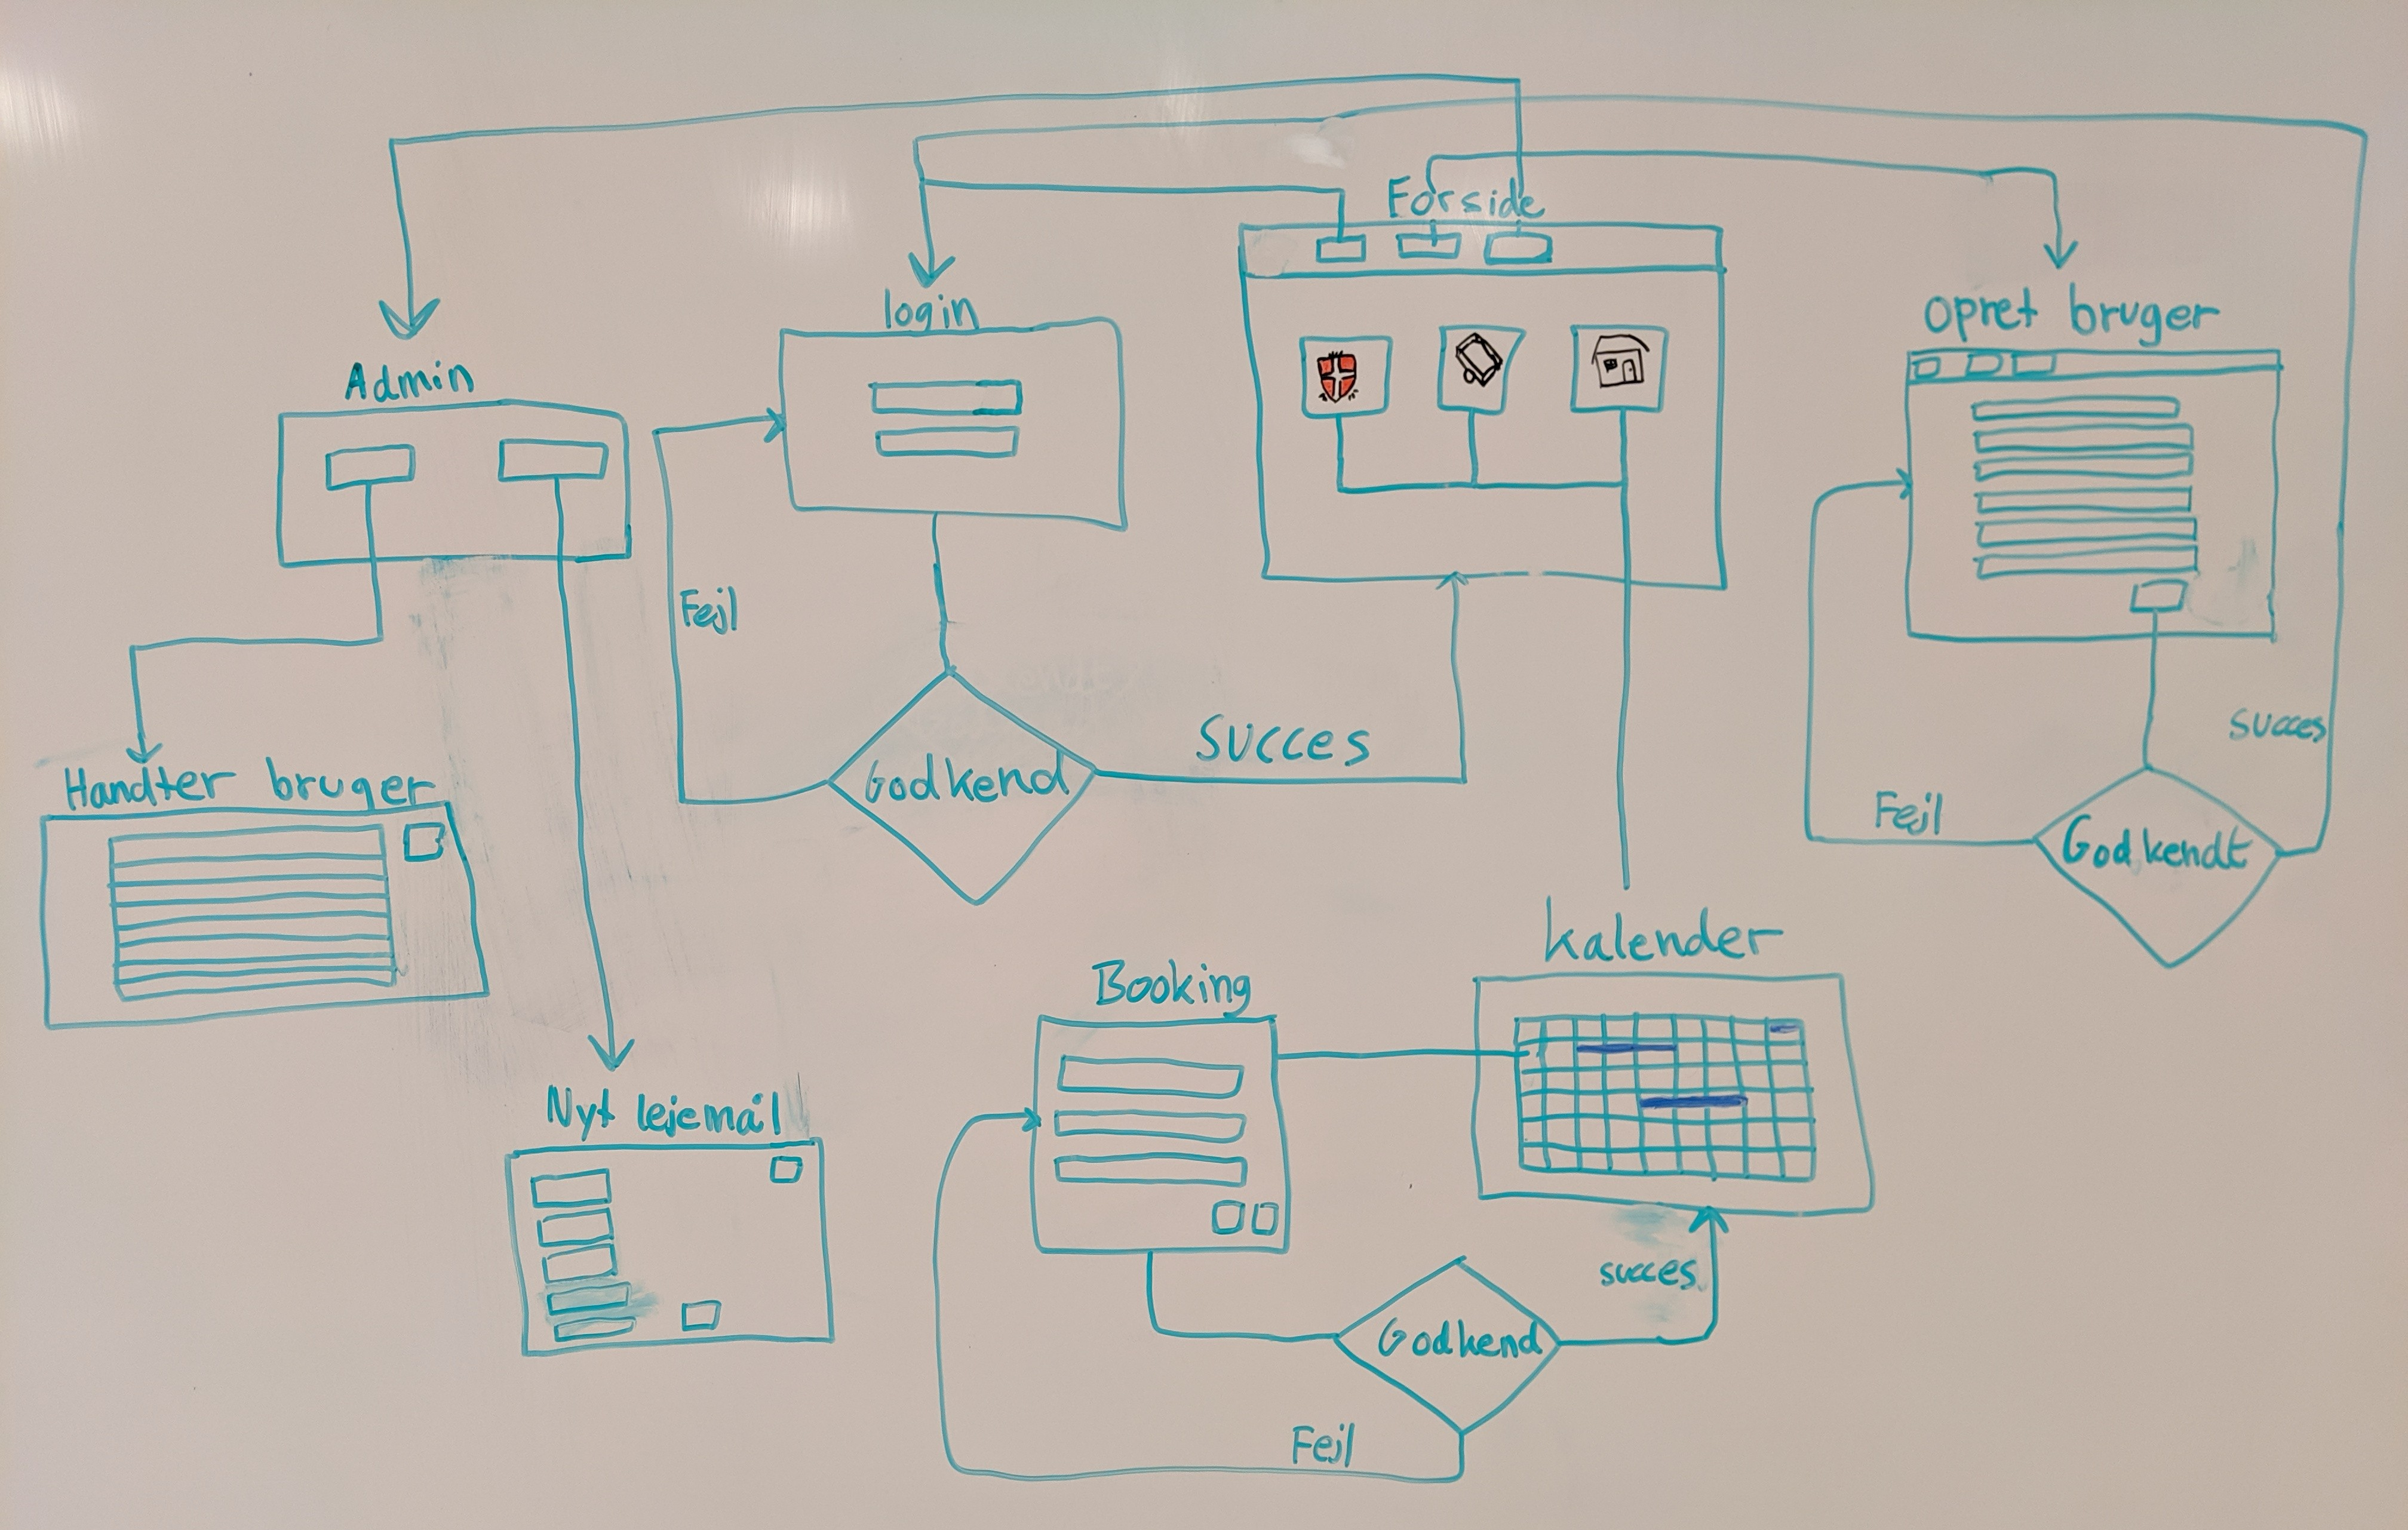
\includegraphics[scale=0.151, angle = 90]{Billeder/Diagrammer/userflow.jpg}
    
    
    \section{Skema diagram og database struktur}
    \chapterauthor{Philip B.Ø (s185137)}
    \noindent Herover ses vores skemadiagram. Da vores hjemmeside giver mulighed for booking, skal vi have et sted hvor vi kan gemme bookings. Til dette bruger vi en mysql database til at holde styr på bookings men også lejemål og brugere af vores hjemmeside. Skemadiagrammet viser hvilke dele af vores database der har relationer imellem hinanden, samt hvilke datatyper vi har med at gøre i databasen.
    
     \hspace*{2cm}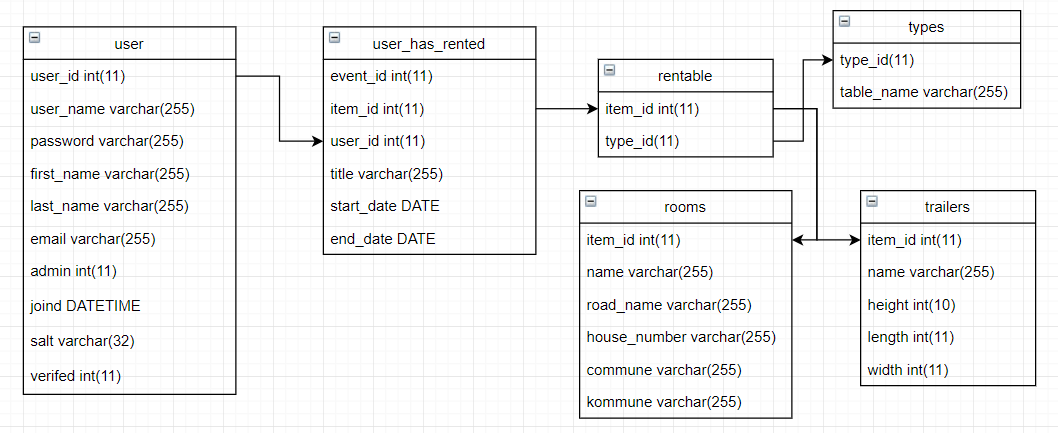
\includegraphics[scale=0.89,angle =90]{Billeder/Diagrammer/SkemaDiagram2,1.PNG}
     
     
     \section{Sekvensdiagram over login process}
     \chapterauthor{Anders R.R (s185146)}
     
     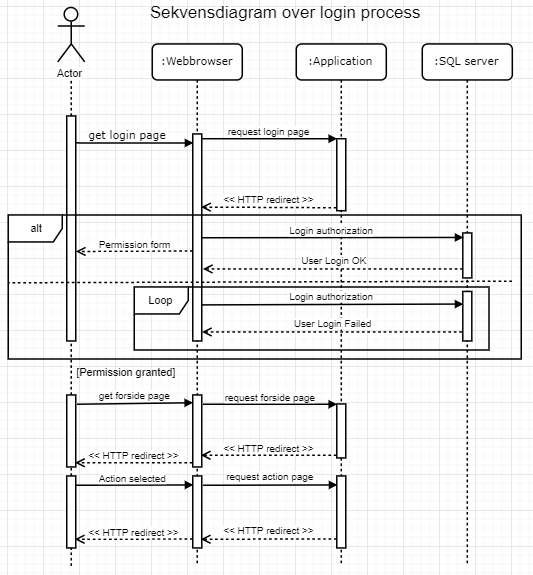
\includegraphics[scale=1.4]{Billeder/Diagrammer/sekvensdiagram.png}
    
    \chapter{Implementering}
    \chapterauthor{William D (s173792)}
    Vi har i denne opgave valgt at skrive vores projekt i PHP, i stedet for Java.
    \newline PHP er et server-side scripting language, som udelukkende bruges til web development. PHP blev udgivet for første gang i 1995, og siden da er der sket stor udvikling inden for sproget. De nyere versioner af PHP har fuldt ud implementeret et Objekt-orienteret programmeringsparadigme, og derved er PHP blevet til et sprog, som ligner Java på rigtig mange områder. PHP er det oplagte sprog at bruge, hvis man skal arbejde med web udvikling i et mindre omfang, såsom vi gør i CDIO. PHP er også et programmeringssprog, som er utroligt nemt at komme igang med, sammenlignet med en web-applikation skrevet i Java, som kører på en Tomcat server. 
    
    \section{Java vs PHP}
    \chapterauthor{Anders B.P (s185129)}
    Der findes dog stadig store og betydningsfulde forskelle imellem PHP og Java. PHP er et typeless programmeringssprog, hvilket vil sige at man som programmør ikke definere typer i PHP, hvorimod man i Java altid skal definere typerne på variabler. 
    Derudover startede PHP i sin tid som en procedual programmeringssprog, men i nyere versioner er der fuldt implementeret objekt-oritenteret programmering, hvilket også gør at PHP syntax faktisk ligner utroligt meget den af Java. 
    Den helt store forskel på Java og PHP når det kommer til web-udvikling, ligger i at PHP er et udelukkende server-side scripting language. Dette har en helt klar fordel, når man arbejeder med et forholdsvist lille projekt, som vi jo gør i dette tilfælde. PHP gør det nemmere at udvikle kode hurtigt, da det generalt kræver en del færrere linje kode. PHP kører på sin egen CGI (common gateway interface), hvorimod, hvis man arbejder med Java kræver det en del ekstra kode at arbejde med en Tomcat webserver. 
    Endnu en forskel er hvordan man præsentere de to typer filer i sin browser. Ofte brugt til PHP er XAMPP, der er en kollektion af web services, der kan håndtere requests fra port 80/443 (Apache), Databaser (MySQL) og Server Side Processing (PHP). Java benytter siger af Tomcat, som er en web services til at hoste Java aplikationer, hvor man deployer en .WAR-fil. 
    
    \subsection*{Java vs PHP i CDIO3}
    \chapterauthor*{Nicklas C.F (s180087)}
    I HTML der kan man lave en form, der har en action attribut der kan sende form-parametre videre til en php-side. PHP-siden kan selv skabe forbindelsen til databasen, lave statements, SQL-queries, sende HTTP requests og modtage en response, med de informationer den fik fra HTML-siden samt vende tilbage til HTML-siden vha sin header. Med andre ord kan PHP tage sig af rigtig meget. For at lave en simpel bruger og sende dataen til en database er kun 2 filer nødvendig. En HTML-fil og en PHP-fil. Ingen dependencies eller imports/includes er nødvendige. 
    
    I Java skal der flere "hop" til. Man skal lave en UserDTO og UserDAO, som er de klasser i java der er ansvarlige for at sende dataen ned i databasen. For at lave SQL-queries skal vi importe sql i java. Da vi jo kører med REST, laver vi en pakke(kaldet rest) der indeholder en Appconfig-klasse, samt en service-klasse. rest-pakken og appconfig er for at skabe "paths" til metoder til håndtering af HTTP requests. For at kunne bruge @GET, @POST. @Path osv. importere vi Jersey API. Fra vores HTML til rest, kan vi i heldige situationer sende direkte fra vores form's action attribute, men i mere kringlede situationer skal vi benytte os af JavaScript+jQuery+AJAX, så endnu mere vi skal importere. Metoderne i rest-service-klaseen sender så informationerne videre til UserDAO'en eller sender et JSON objekt tilbage (alt efter hvad vi ønsker). Til sidst skal vi også huske at have JDBC driver i form af MySQL-connector depedency og samtidig lægge en .jar af samme connector i Tomcats WEB-INF/lib folder så der er database adgang. 
    
    Så for at opsummere hvor meget man skal bruge i de to for at skabe en bruger i en database: \\
    \begin{itemize}
        \item PHP version
        \begin{itemize}
            \item HTML fil
            \item PHP 
            \item XAMPP
        \end{itemize}
        \item Java version
        \begin{itemize}
            \item HTML fil
            \item Java fil(er)
            \item Tomcat + .WAR fil
            \item Jersey API
            \item SQl import + JDBC driver(MySQL Connector) + connector-jar i Tomcat
            \item JavaScript + jQuery + AJAX + JSON
        \end{itemize}
   
    \end{itemize}
    
    \noindent Selvølgelig skal man ikke i alle situationer benytte sig af alle disse imports og man designer selv, men i vores implementering benytter vi os af det hele.
    
    
    \section{Valg af database}
    \chapterauthor{Michael J. (s185123)}
    Vi har i dette projekt valgt at arbejde med en MySQL database. Grunden til dette er at vi i tidligere kurser har stiftet kendskab med specifikt MySQL, og derudover er MySQL en relationel databasestruktur, hvilket egner sig godt til vores projekt da vi både har en bruger der kan have forskellige roller, men også forskellige lejemål, som f.eks. både optræder som en trailer eller mødelokale. Selve vores databasestruktur er opbygget så vi nemt kan tilføje eller udvide med nye lejemål, brugere eller flere forskellige roller. Dette resultere i at det i princippet er ligegyldigt, om vi har 2 eller 100 lejemål, og derudover er det også nemt at tilføje f.eks. en båd, hvis FDF-klubben ønsker at tilføje flere forskellige lejemål af andre kategorier end bare trailere og mødelokaler. 

    \section{Sikkerhed}
    \chapterauthor{Michael J. (s185123)}
    Da vi i dette projekt udvikler en web-applikation til en reel kunde, har vi selvfølgelig også været nød til at tage sikkerhed med i vores overvejelser, når det kommer til håndtering af passwords, cookies, session og ikke mindst vores database queries. 
    
    \subsection*{Passwords}
    \chapterauthor*{Michael J. (s185123)}
    Først og fremmest er vi nød til at håndtere passwords korrekt. Måden vi gør dette på er at generere en 'salt' via en metode salt(), som PHP stiller til rådighed for os. Derudover hasher vi passwordet ved hjælp af en Secure Hash Algorithm kaldet sha-256. Vi gemmer derefter det hashede password+salt, samt den tilfældigt generede salt i databasen. Grunden til at vi anvender en salt, er fordi hashing af passwordet i sig selv ikke er en sikkermåde at opbevarer passwordet på, derfor tilføjes en salt, som bare er en lang pseudorandom String, til passwordet. 
    
    \subsection*{MySQL Queries}
    \chapterauthor*{Michael J. (s185123)}
    I dette har projekt har vi anvendt en MySQL database, dette betyder selvfølgelig også at vi er nød til at sikre os imod SQL-injections. Dette gøres ved kun at benytte prepared statements hele vejen igennem vores kode. Når vi i vores kode anvender prepared statements betyder det at vi bruger 'bound parameters', og dette gør at vores database server først compiler vores querie, og når vi kalder execute metoden, bliver vores prepared statement binded med vores parametre. Dette resultere i at vores brugere ikke kan indtaste ondsindede strings eller lign. som kan have effekt på vores database.
    
   \subsection*{Sessions}
   \chapterauthor*{Michael J. (s185123)}
   Vi har i dette projekt anvendt sessions til at holde en bruger logget ind på tværs af vores forskellige hjemmesider indtil brugeren forlader vores domæne. Den måde sessions fungerer på i PHP, er ved at generere en 16-byte lang unik identifikations string. Denne streng bliver gemt hos clienten i en cookie, og samtidig bliver den også gemt på webserveren. Hvergang brugeren så navigerer rundt på vores domæne vil der ved hvert request blive sammenlignet klientens cookie opmod vores webservers sessions id's, og hvis der er et match kan vi genkende brugeren. Sessions er en sikker måde at gøre vores hjemmeside statefull, i det at vores session id bliver opbevaret på selve vores webserver, sålænge vores webserver er sikker vel og mærket. 
    
    
    
    \section{Struktur af kode}
    \chapterauthor{William D. (s173792)}
        Vi har udarbejde vores kode ud fra princippet om at holde det objektorienteret. Når man arbejder med php har man mulighed for at gøre begge dele, men den objektorienteret vej er noget mere læsbar og fylder ikke lige så mange linje kode. 
        
        Vi har opbygget vores kode på en sådan måde at vi i starten af alle vores php filer require once en init fil, som svare til at importere den. Vi har så to typer af .php filer, selve web-siderne og klasse filerne. Til alle sider som har en speciel funktionalitet har vi lavet en seperat klasse dertil, og så har vi lavet nogle underliggende klasser til brug i andre, f.eks. Database-klassen. De klasser vi har i vores projekt er følgende:
        \begin{itemize}
            \item AdminHandler
            \item Config
            \item CreateItem
            \item Database
            \item Events
            \item Hash
            \item Input
            \item Redirect
            \item Session
            \item User
            \item Validate
        \end{itemize}
        Af disse klasser er der 3 overordnet kategorier: Statiske hjælper-klasser, Instance hjælper-klasser og Funktionalitets-klasser. 
        \newline\newline De statiske hjælperklasser er: Config, Hash, Input, Redirect, Session.
        \newline Instance hjælper-klasserne er: Database, Validate.
        \newline Og Funktionalitets-klasserne er: AdminHandler, CreateItem, Events, User.\par
        \noindent Generelt gør de statiske hjælpeklasser det at de Læser information fra et fast sted og giver det, f.eks. vores Config klasse læser fra vores config-fil og giver det vidre til de andre klasser der beder om det.\par
        \noindent Instance hjælpe-klasserne gør det at der oprettes et instance af dem og så har de metoder til at håndtere en ting, for validate er det at validere det input der er givet til den ud fra en række krav givet til den og så retunere den en række fejl eller en sucess. Database-klassen har metoder til at gøre kommunikation til databasen let, såsom getAll(table), eller get(table, requirement)\par
        \noindent Funktionalitets-klasserne har alle sammen hvert ders ansvarsområde.\newline
        AdminHandler står for alt den funktionalitet en administrator i systemes skal have, primært håndtering over andre brugere.\newline
        CreatItem bruges til at oprette nye kategorier af hvad der kan udlejes og og nye ting der kan udlejes i de kategorier.\newline
        Events bruges til at oprette nye udlejninger og vise dem der er i databasen.\newline
        User er den mest speciele klasse vi har, den står selvfølgelig for at brugerhåndtering, login, logud, få brugere i systemet, men den står også for at gemme den bruger der logger ind i en session i en seperat klasse, så den har i sig hvad der minder om en sub-class som bliver gemt for at hjemmesiden ved man er logget ind.
    
    \chapter{Test}
    \chapterauthor{Nicklas C.F (s180087)}
    
    \section{Bruger test}
    i forbindelse med vores projekt har vi udviklet nogle brugertests. Vores projekt skal reelt ud på markedet og skal benyttes af brugere der ikke er gode til at omgås en computer. Derfor var det vigtigst for os, at vores hjemmeside var intuitiv og let tilgængelig. Det var vores fokus punkt i vores test cases i form af at det er opret bruger/login og booking/kalender vi har i fokus. Funktioner og operationer som kun kan tilgås af en admin (dvs os) er ikke blevet testet af brugere.
    En blank brugertest er vedhæftet som bilag.
    
    Respons fra brugertests:
    

\noindent\textbf{Brugertest respons:} I kalenderen kan alle brugere redigere alle bookingerne

\noindent\textbf{Vores modsvar:} Denne bug var vi godt klar over på det gældende tidspunkt. Det er blevet rettet således at det kun er brugeren der har oprettet bookingen (og selvfølgelig også admins) der kan redigere og slette bookingen.

\noindent\textbf{Brugertest respons:} Hvis man klikker på en oprettet booking (det blå stykke) går direkte ind på redigering.

\noindent\textbf{Vores modsvar:} Denne bug var bundet op på den overstående og vi var også godt klar over den. Som sagt er det nu kun opretshaveren/admins der kan tilgå en booking.

\noindent\textbf{Brugertest respons:} Det er svært at kende forskel på trailer-bookings og hytte-bookings på kalenderen hvor man kan se alle bookings.

\noindent\textbf{Vores modsvar:} Vores originale plan var at trailer bookings og hytte-bookings skulle være hver sin farve i kalendereen, fx trailere var røde og hytter blå. Vi har dog problemer med at få det implementeret men arbejder på sagen. Bliver ikke implementeret før efter CDIO.

\noindent\textbf{Brugertest respons:} Det ville være godt at have en profil-side, hvor man kan se sin profil og evt ændre oplysninger.

\noindent\textbf{Vores modsvar:} Enig. Vi belyser dette i vores afsnit om forbedringer

    \section{unitTest}
    Der findes PHP-frameworks til at lave unitTest i PHP. Men det er lidt "uncharted territory" for os, for hvilket frameworks skal man bruge til hvilken form for tests. Desuden er det mest det grafiske og intuitive der er det vigtigste i forbindelse med projektet, så vi følte at brugertests var bedre brug af vores tid end unittests.
    \newline Med det sagt, så ville det have været fornuftigt at opsætte unitTests med nogen mock-klasser, der kunne simulere vores database, og derved teste funktioner såsom login, opret burger, log ud osv. Vi valgte dog her, som sagt, at fokusere på at lave nogle brugertests da vi følte at vores front-end var vigtigere at få testet grundigt, iforhold til at vores målgruppe ikke er særlig tech-savy, og derved sætter pris på et minimalt og simpelt design. 

    
    
    \chapter{Fremtidige forbedringer}
    \chapterauthor{Anders B.P (s185129)}
    Vi har i dette projekt et par ønskede funktioner, som vi desværre ikke har fået implementeret. Vi havde et ønske om, at man på forsiden skulle kunne danne sig et overblik over hvilke lejemål der er ledige i en bestemt periode via en søging/filtrering metode. Dette har vi ikke fået implementeret, i stedet er brugeren nød til at klikke ind på selve kalenderen og bladre igennem de forskellige uger/måneder, for at finde ud af hvornår forskellige lejemål er ledige. Det mest optimale ville være, hvis en bruger blot kunne vælge en kategori for et lejemål, f.eks. trailer, og derefter vælge en dato for udlejning, hvorefter vores søgefunktion automatisk ville finde hvilken somhelst ledig trailer i den givne tidsperiode.
    Dette vil helt klart gøre brugeroplevelsen nemmere, simplere og hurtigere. 
    \newline Derudover ønskede vi også en nem måde for en administrator at filtrer eller søge, efter medlemmer i databasen. På nuværende tidspunkt bliver alle brugere i databasen vist under administratorens brugerhåndtering, hvilket hurtigt kan blive uoverskueligt, kommer der mange brugere. 
    \newline Herudover ønskede vi også en side, hvor en bruger ville kunne se sin egen profil. Dette har vi desværre heller ikke kunne implementere i tide. Meningen med denne side var at brugeren skulle kunne se sin egen profil, og rette i alle hans oplysninger, hvis f.eks. et telefonnummer ændredede sig. Vi besluttede ikke at fokusere på denne del, da administratoren blot kan slette brugeren og derefter kan brugeren oprette en ny profil med de nye oplysninger. 
    \newline Til sidst var vores plan også at have en side hvor en administrator ville være i stand til at ændre oplysninger om de enkelte lejemål. Dette har vi også valgt at undlade at implementerer i denne omgang. Vi har dog opret- og slet lejemål funktionen på plads, så her kan en administrator også slette et lejemål, og derefter oprette en ny med de opdaterede oplysninger. 
    \newline Alt i alt mangler vores hjemmeside et par quality-of-life funktioner, som vil forbedre brugervenlighed, men vi ser disse funktioner, som værende ikke kritiske overfor den overordnede funktion af vores hjemmeside. 
    
    
    \chapter{Konklusion}
    \chapterauthor{Anders R.R (s185246)}
    
    
    \noindent Siden at vi har valgt ikke at lave standard projektet har der været en masse ekstra som skulle formuleres end blot påbegyndelse og udarbejdning af design. Vi har taget lange dialoger med vores kunde omkring de rammer og den vision, som der skulle skabes for projektet og konverteret dem til en lang liste krav og usecases som ville være relevante at få indført.
    
    \noindent For at opnå det bedste resultat for kunden har vi fokuseret på de use-cases, som vi følte var mest relevante for vores slutbruger. Siden at vores slutbruger ikke er vant til teknologi, har vi lagt stort fokus på simplicitet og tilgængelighed. Vi har prioriteret at kunden for det best mulige projekt, fremfor at fremskynde bestemte features til at præsentere dem til eksamen. 
    
    \noindent Alt i alt er vi tilfredse med projeket i og med at kerne funktionerne er implementeret og fuldt funktionelle og vores design er intuitivt. Vi ville gerne have haft mere fokus på at opbygge nogen solide rammer for at teste selve vores kode, men vi valgte her at fokusere på at teste vores front end på bekostning af test af vores back end. Derudover mangler vi at implementere et par use-cases, som ikke er kommet med i denne omgang, men som vi forsætter med at udvikle videre på i fremtiden. 

    \begin{appendix}
    \chapter{Test cases}
    \begin{figure}
    \centering 
    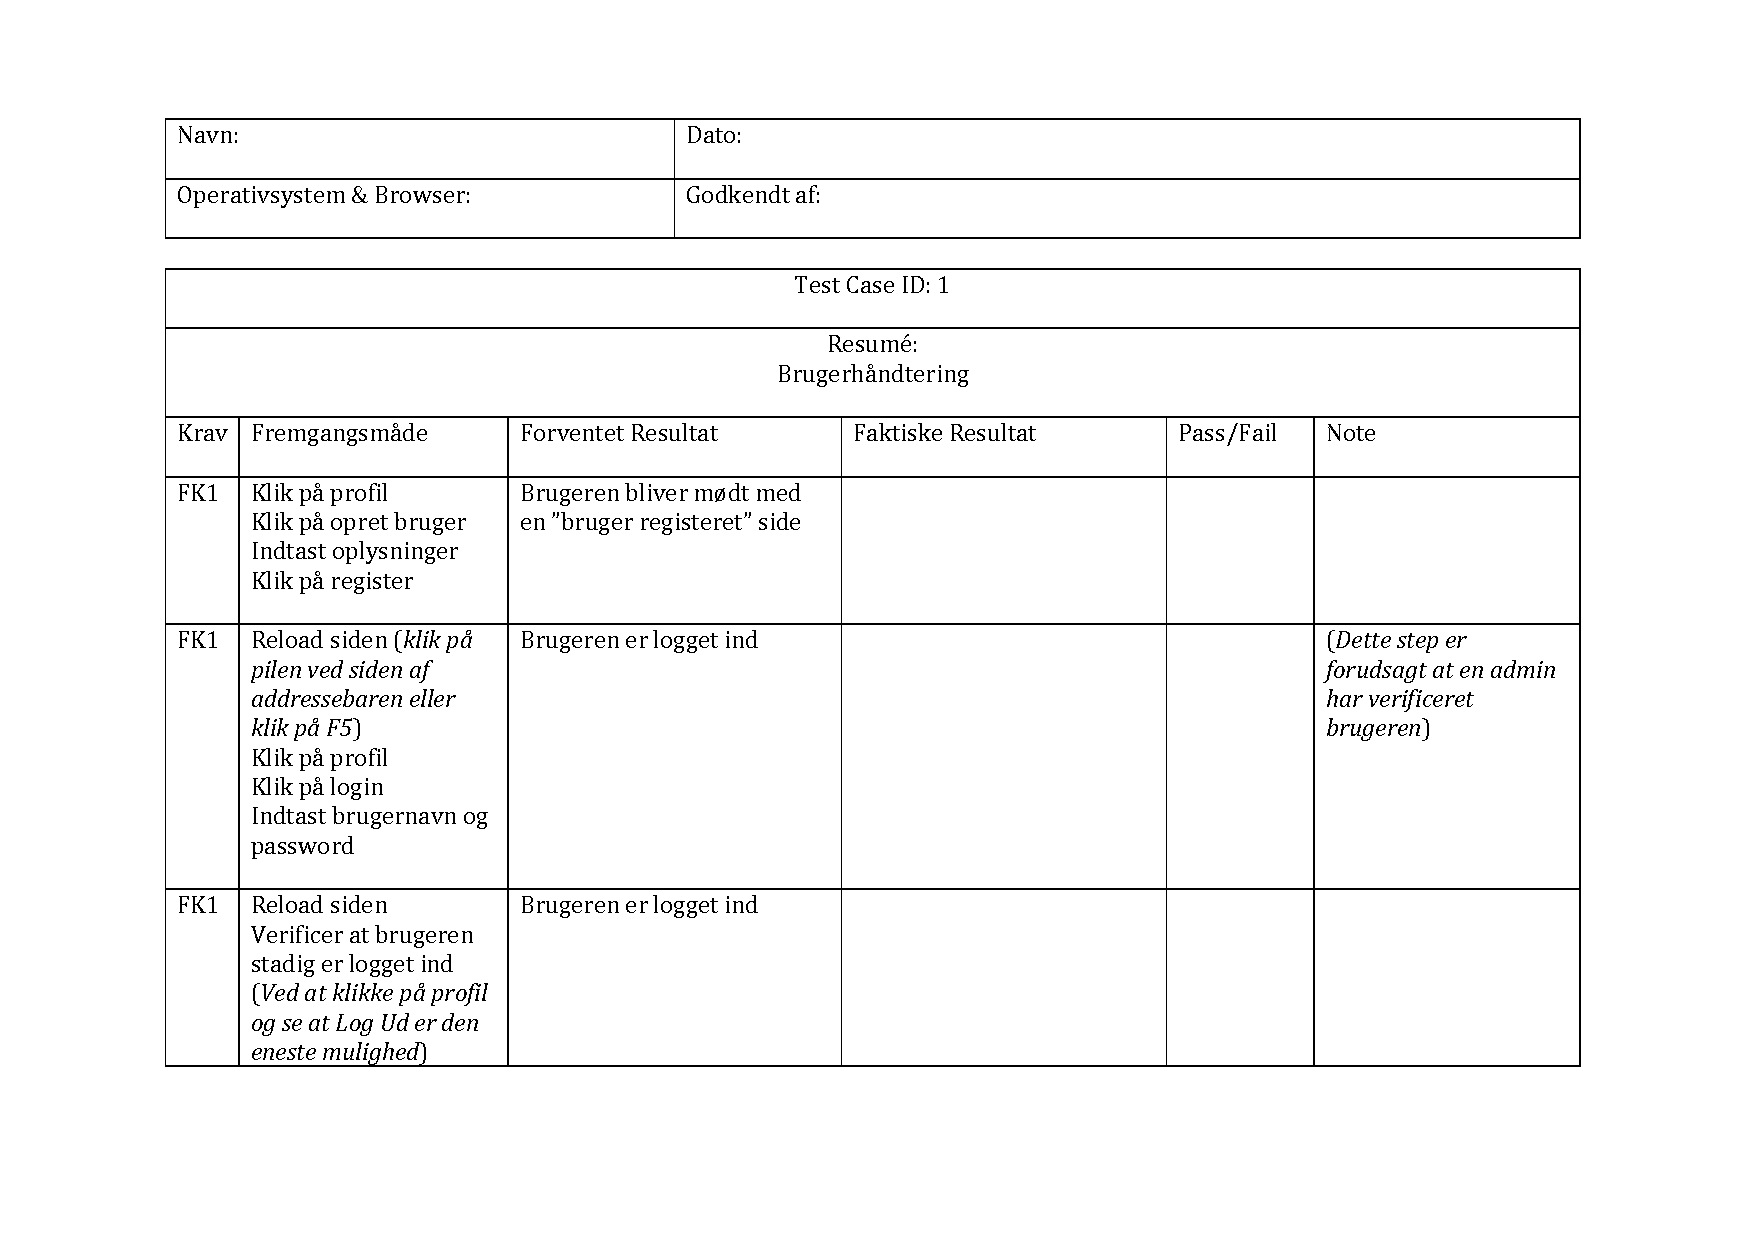
\includepdf[]{Billeder/Bilag/testCases.pdf}
    \end{figure}
    \end{appendix}
    
    \chapter{Disposition for fremlæggelse}
    
    \begin{itemize}
        \item \textbf{Indledning}
        \begin{itemize}
                \item Indledning (Anders BP)
                \item vision (Philip)
                \item krav og usecases (Anders BP)
             \end{itemize} 
        \item Diagrammer
        \begin{itemize}
                \item Bruger flow (Anders E og Philip)
                \item Skema diagram (Philip)
                \item Sekvensdiagram (Anders E)
             \end{itemize} 
        \item Demonstrering af produkt. (ansvar: forklarer: Anders E og Philip ) 
        \item  Java vs PHP (generelt)
        \begin{itemize}
                \item generelt / forskel (ansvar: Anders BP)
                \item Cdio3  / (vores projekt) (ansvar: Nicklas)
             \end{itemize}
        \item \textbf{Implementering}
            \begin{itemize}
                \item Valg af database (Philip)
                \item Sikkerhed (Michael J.)
                \item Sessions (Michael J.)
             \end{itemize}
        \item \textbf{ Struktur af kode} 
            \begin{itemize}
                \item AdminHandler (ansvar: Michael J.)
                \item Config (ansvar: William D ) 
                \item CreateItem (ansvar: Michael J.)
                \item Database (ansvar: William D ) 
                \item Events (ansvar: William D ) 
                \item Hash (ansvar: Michael J.)
                \item Input (ansvar: William D ) 
                \item Redirect (ansvar: William D ) 
                \item Session (ansvar: Michael J.)
                \item User (ansvar: William D ) 
                \item Validate (ansvar: William D ) 
             \end{itemize} 
         \item Test (ansvar: Nicklas)
        \item \textbf{Konklusion}  (ansvar: Dobbelt A) 
            \begin{itemize}
                    \item Manglende use-cases
                    \item Krav ikke opfyldt
                    \begin{itemize}
                        \item 
                        Rediger egen brugerprofil
                        \item
                        Administrator kan kun redigere Password
                        \item
                        Slet egen bruger
                        \item
                        Alle brugere kan slette alle bookinger. (bør kun være administrator og brugeren som har lagt reserveringen)
                        
                 \end{itemize}
                    \item Fremtidige forbedringer (Anders BP)
                    \begin{itemize}
                        \item Sikkerhed
                        \item filtreret søgning
                        \item Dynamisk forside
                    \end{itemize}
                    
                    \item UnitTests (Anders BP)
                    \item 
                 \end{itemize}
            
        
         
    \end{itemize}
    
    
    
\end{document}